\section{Methodology}\label{sec:methology}

\subsection{Dataset}\label{subsec:dataset}

In our project, we utilized the \emph{Human Activity Recognition Using Smartphones} dataset, referenced in our literature as~\cite{misc_human_activity_recognition_using_smartphones_240}.
This database is built from recordings of 30 subjects performing activities of daily living (ADL) while carrying a waist-mounted smartphone with embedded inertial sensors.

It was sourced from a diverse group of 30 volunteers aged 19--48, the dataset captures six common activities: walking, walking upstairs, walking downstairs, sitting, standing, and laying.
Each subject wore a Samsung Galaxy S II smartphone on the waist, enabling the capture of 3-axial linear acceleration and 3-axial angular velocity at a 50Hz rate.
The dataset, a multivariate time-series collection in the computer science domain, is suitable for tasks such as classification and clustering.

Instead of the raw time-series data, we utilized the processed features of the \emph{Human Activity Recognition Using Smartphones} dataset.
The dataset provided a comprehensive set of features derived from the accelerometer and gyroscope sensors, which were more aligned with our project objectives.

These features include various statistical measures estimated from the processed sensor signals such as but not limited to mean, standard deviation, median absolute deviation as well as frequency domain features derived from the Fast Fourier Transform (FFT).
In total, the dataset provided 561 features for each sample.
Which of these features were used in our project is discussed in Section~\ref{subsec:preprocessing}.

The authors of the dataset also provided a partitioned dataset, which was split into two sets: a training set and a test set.
The training set consists of 70\% of the data, while the test set consists of the remaining 30\%.
Which comes to 7352 and 2947 samples respectively.


\subsection{Preprocessing}\label{subsec:preprocessing}

Since the dataset was already processed, we did not have to perform any preprocessing steps to generate features, but we did some preprocessing to reduce the number of features.

% TODO search for paper to reference for correlation matrix

For this we used a correlation matrix to find features that were highly correlated with each other.
Features that have a high correlation with each other, imply that they are redundant and can be removed.
Redundant features can be removed, since the information they provide is already captured by other features.
This reduces the number of features, which in turn leads to models that are less complex, as they need to learn fewer features.

Figure~\ref{fig:cormat-before} shows the correlation matrix before preprocessing, while Figure~\ref{fig:cormat-after} shows the correlation matrix after preprocessing.
As a threshold for removing features, we used a correlation coefficient of \emph{0.95}.
This reduced the amount of features from 561 to 253, effectively reducing the number of features by more than half.

\begin{figure}[ht]
    \centering
    \begin{minipage}{0.45\textwidth}
        \centering
        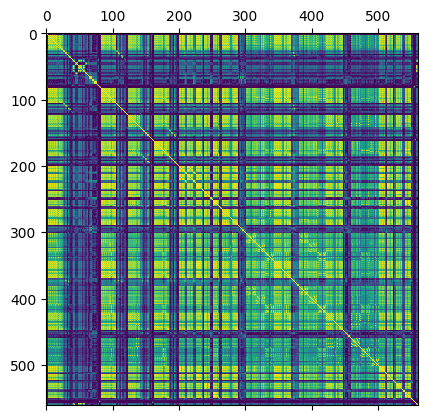
\includegraphics[width=\textwidth]{./img/correlation-matrix-before}
        \caption{Correlation matrix before preprocessing}
        \label{fig:cormat-before}
    \end{minipage}\hfill
    \begin{minipage}{0.45\textwidth}
        \centering
        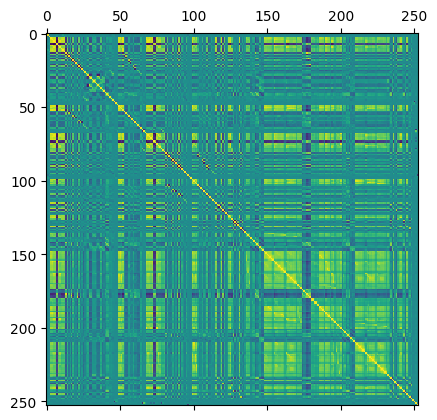
\includegraphics[width=\textwidth]{./img/correlation-matrix-after}
        \caption{Correlation matrix after preprocessing}
        \label{fig:cormat-after}
    \end{minipage}
\end{figure}

We also decided to use the test set provided by the dataset as our held-back test set.
For training, we split the training set into a set used for actual training and a set used for validation.
This was done to be able to evaluate the performance of the model during training, and to ensure that the model did not overfit to the training set.
The validation set was 30\% of the training set, which comes to around 2206 samples for the validation set and 5146 samples for the training set.

\subsection{Architectures}\label{subsec:architectures}

This section discusses the architectures we tried and evaluated in our project.
For different architectures we tried to first build a simple model, and then a more complex one that where we also tuned the hyperparameters.

\subsubsection{Feedforward Neural Network}

\textbf{Simple Feedforward Neural Network}

Our project initiated with a simple Feedforward Neural Network (FF).
This model consisted of an initial dense layer with 512 units, a hidden dense layer with 128 units using the ReLU activation function, and an output dense layer with 6 unit.
This was the simplest model we could think of.

\textbf{Tuned Complex Feedforward Neural Network}

The results from the simple Feedforward model were not satisfactory, so we decided to build a more complex model and tune it.
For this we utilized Keras Tuner, employing a RandomSearch strategy.
This approach allowed us to automatically fine-tune the hyperparameters of our model, such as the number of layers, the number of units in each layer, the dropout rate, and the learning rate.
The goal was to identify the most effective configuration for our dataset, enhancing the model's performance.

\subsubsection{Convolutional Neural Network}

\textbf{Simple Convolutional Neural Network}

We also developed a Convolutional Neural Network model, comprising convolutional layers, max pooling, global max pooling, a dropout layer for regularization, and a softmax output layer.
While such models are typically used for image classification, we wanted to explore whether they could be used for time-series classification as well.
This also did not need any real preprocessing apart from reshaping the data to fit the input shape of the network.

\textbf{Tuned Complex Convolutional Neural Network}
While the simple Convolutional Neural Network model performed well, we still wanted to explore whether we could improve its performance by tuning its hyperparameters.
This involved tuning the number of filters in the convolutional layers and the dropout rate.



